\section {Video Selfie}
The first question we ask about this dataset, to understand the contribution of human affects was, is there any such thing as a video selfie. The paper by Bakshi et.al \cite{Bakhshi:2014:FEU:2611105.2557403} shows that faces in an image play a major role in popularity of that image on instagram. Our aim is to see whether a similar behaviour exist in video social networks like Vine. For this , we had to first plot some statistics regarding how many of the collected vines contain faces amongst the major fraction of the video frames. We would define these videos as video-selfies, or videos that potentially mimic still selfie like behaviour. To understand this better, we processed each video using the well known framework for face detection by Viola and Jones \cite{Viola:2004:RRF:966432.966458} to detect profile and frontal faces in a video. We collected these measurements across all the collected vine videos and stored the face frames as well as the statistics of each video. After plotting the CDFs of the ratio of face frames to total frames for all videos \ref{fig:CDF_Compound}, we found that more than 50 percent of popular vines which ranked in top 100, had the ratio to be more than 0.5. The mean ratio of face frames to total frames was 54.74 percent, across all the collected samples. Further we plotted the distribution of these ratios as shown in \ref{fig:faceratio_destribution}. These numbers indicate that there is a similar phenomenon like still selfies , prevalent on video social networks like vine. 

\begin{figure}
\centering
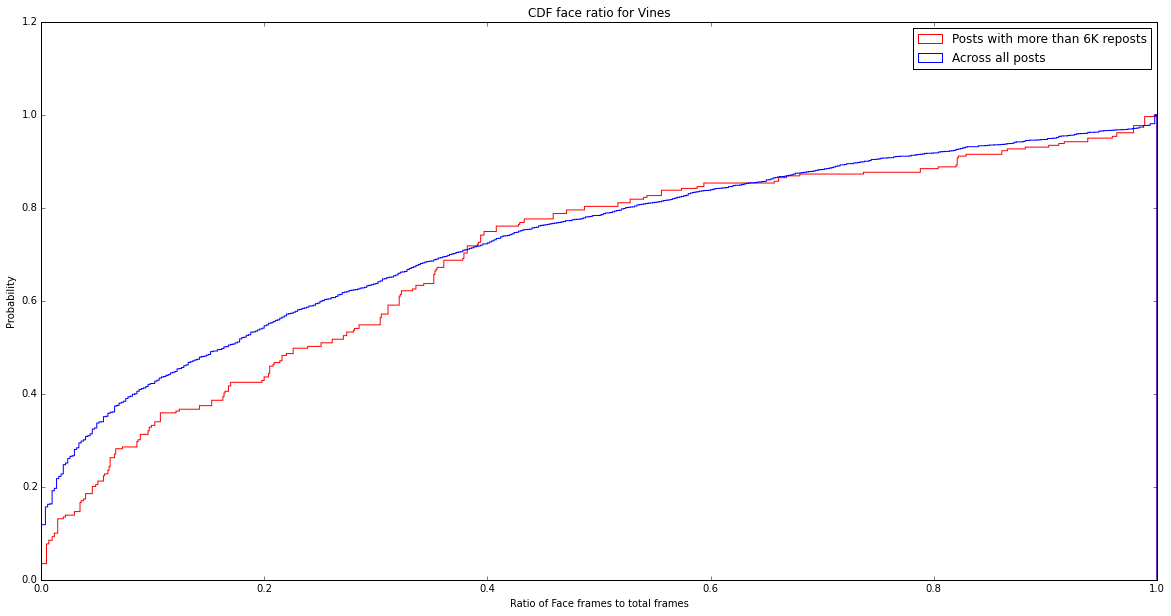
\includegraphics[width=\columnwidth]{plots/CDF_Compound}
\caption{\textbf{CDF of Face frames to total frames calculated for Frontal and Profile faces }}
\label{fig:CDF_Compound}
\end{figure}

\begin{figure}
\centering
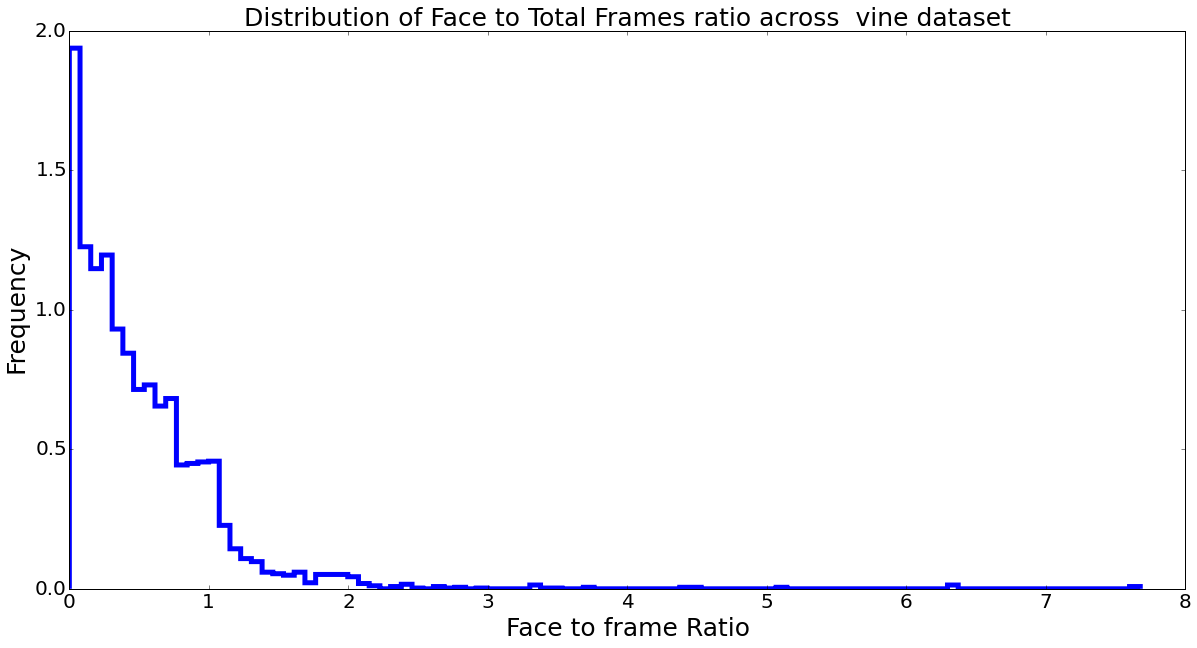
\includegraphics[width=\columnwidth]{plots/faceratio_destribution_dataset}
\caption{\textbf{ Distribution of face frames compared to total frames for all the Vine videos in the dataset}}
\label{fig:faceratio_destribution}
\end{figure}
